\chapter{Setting up a Star Cluster}

\section{A Model for a Star Cluster}

\abc

\bob
Now we have a nifty N-body integrator.  So what shall we do with it?

\carol
So far, we have only worked with two or three stars.  How about
throwing in a whole bunch?

\bob
Fine, but we have to decide how to set them up.
We can't very well put them all on a circle.  It wouldn't be
stable anyway, as we have seen already with three particles.

\carol
I can't think of any other particular pattern either.  Perhaps
we should just pick random positions.  But random within a certain
region, I suppose, not all over the universe, since then they wouldn't
interact.

\alice
How about letting nature guide us, and constructing a very simple
model for a star cluster.  Let us assume that a group of stars are
born together in a small corner of a galaxy.

\bob
Sounds good.  How shall we model that?

\alice
It would be simplest to group the stars in a sphere, and so assume a
homogeneous distribution, i.e. constant density.  In the general case,
we should assign each star not only an initial position, but also an
initial velocity.  Let us again start with the simplest possible
assumption, namely that of zero velocities for all stars.  In other
words, all stars are born at rest.

\carol
Wouldn't they all start falling to the middle, right away, under the
influence of their mutually attractive forces of gravity?

\bob
I would think so.  That means that the system will shrink at first.
But what will happen next?  Will it shrink forever, or start
expanding, or oscillating, or what?  We will have to do real
experiments to find out.

\carol
First we have to construct the initial state, as described above.  We
have to introduce a random number generator, and then use that to
choose a random position within a sphere.  We may as well choose
coordinates such that we will start with a sphere of unit radius.

\cba

\section{Implementation: a Sphere in Cold Start}

After a lengthy session, our friends came up with a code, tentatively
called {\st sphere1a.C}.  Having had the experience of writing the
{\st nbody\_sh1.C} code, it was not to heard to write the bulk of the
code, with the {\st main} driver, the output routine, and so on.  The
only really new ingredients were the random number generator and the
function {\st sphere} that gave all particles their initial conditions.

\abc

\alice
Well, I think we did a nice job.  We're beginning to get good at this!

\bob
Yes, it's a lot less daunting that I had thought.  Once you have one
moderately complex code written and tested and documented, it gets a
lot easier to write the next one.  You can simply start with what you
already have, and make a variation.

\carol
You mentioned documentation.  We have written comments here and there,
and at the head of each function, but perhaps we should get into the
habit of providing a little more information, as an introduction, or a
form of primer or manual, besides the code comments themselves?

\bob
By our guest!

\alice
Yes, I think you should do that, Carol.  After all, you are supposed
to have learned all that good stuff in your classes!

\carol
So much for making a good suggestion, only to get saddled with the work.
Oh well, I actually like summarizing what I've done, once I'm happy with
it, so let me give it a try.  I'll keep it short, though, for now.
Here goes.

\cba

We list here the full code for {\st sphere.C}, split up into its
functions.  First the information at the head of the file:

\code{sphere1a.C: summary}{chap9/sphere1a.C.1_summary}

This comment block is followed by the {\st \#include} directives and
other general definitions, and then the declarations of all functions.

\code{sphere1a.C: premain}{chap9/sphere1a.C.2_premain}

In the {\it main\ } function, the reader is asked to provide a value
for the desired number of particles, and optionally a seed for the
random number generator.  When you want to do a number of independent
runs, it is better not to specify such a seed, since then each run
will receive a different random seed.  If then you want to rerun a
particular run, you can specify the seed that happened to be used in
that run.  You can find the value of the seed used at the beginning of
the output of each run, so even if you did not specify one, you will
still be able to run any run again. 

Note that in reality there is no such thing as a truly random number;
instead we use a pseudo-random number, generated by an algorithm
designed to generate numbers that are (hopefully) random-look-alike
enough for our purpose.  As a technical detail, two runs will only get
a different random seed as long as they start more than one second
apart, since the seed is constructed from the unix clock, read off in
seconds.

\code{sphere1a.C: main}{chap9/sphere1a.C.3_main}

The following function is similar to what we used in the previous
chapter, for {\st nbody\_sh1.C}.

\code{sphere1a.C: read\_options}{chap9/sphere1a.C.read_options}

Here is a pseudo-random number generator, which we took from the
old Unix example, one which returns a real number between 0 and 1.

\code{sphere1a.C: randunit}{chap9/sphere1a.C.randunit}

This more general version of a pseudo-random number generator allows
specification of the upper and lower bounds of the interval.

\code{sphere1a.C: randinter}{chap9/sphere1a.C.randinter}

The following function does all the work, places all $N$ particles
homogeneously distributed in a sphere with radius 1.

\code{sphere1a.C: sphere}{chap9/sphere1a.C.sphere}

The resulting $N$-body system is then ready for output.

\code{sphere1a.C: put\_snapshot}{chap9/sphere1a.C.put_snapshot}

\section{Testing, testing, . . .}

\abc

\bob
Short and sweet, as they say.  But perhaps a bit too short, especially
on explaining how exactly we managed to put particles in a sphere
using a, what did you call it, spherical coordinate system?

\alice
Yes, that is a coordinate system that is a lot more convenient for
dealing with spheres than the usual Cartesian coordinate system is;
the latter would of course be better if we would build a star cluster
with the shape of a box.

\bob
I'd prefer the shape of a diamond over that of a box.  But seriously,
how I am to know for sure that the equations you gave me from your
physics course are actually correct?

\carol
The answer they keep repeating in {\it my} courses: testing, testing, \dots

\bob
Okay, let's just run the program with a few particles, okay?  By just
looking at the numbers we may get an idea of whether we are at least
approximately right.  Alice, you're at the keyboard.  Have a go at it!

\alice
Fine.  How about ten particles?

\cba

\begin{small}
\begin{verbatim}
|gravity> sphere1a -n 10
seed = 1063894860
10
0
0.1 0.4540028492193794 0.3498769522044687 0.7969703663542103 0 0 0
0.1 0.03987844095394553 -0.08119205595973951 -0.6615273048865606 0 0 0
0.1 -0.07696021131813481 -0.8459387776849843 0.3519731575017572 0 0 0
0.1 -0.03159529410632059 -0.2076818100526642 0.7862706899063225 0 0 0
0.1 0.02919115871639223 -0.228846199565124 0.2176806328285098 0 0 0
0.1 0.531084745743273 -0.1003377930427043 -0.05342966914946958 0 0 0
0.1 0.7662014881610754 -0.3620973663404717 0.1670139579482853 0 0 0
0.1 0.2522400702554067 -0.6696003994776 -0.08285809759917392 0 0 0
0.1 0.2785462467572272 0.06099199162060588 0.536196594372378 0 0 0
0.1 -0.510335018159465 0.06233465247130211 0.7635335045998497 0 0 0
|gravity> 
\end{verbatim}
\end{small}

\abc

\bob
At least the velocities are zero, and the position coordinates are
smaller than one.

\carol
And larger than minus one.  So far so good.

\alice
Not only that, if one of the numbers comes close to one in absolute value,
the other numbers are smaller.  Indeed, it seems that the sum of the
squares of the position coordinates is always smaller than unity, as
it should be: the particles neatly lie in a sphere.

\bob
But do they lie homogeneously in a sphere?

\carol
I see large and small numbers, positive and negative numbers, so that
all suggest that things are pretty random.

\alice
Bob is right, we really should check for homogeneity.  Random is not
enough, since a random distribution could still be skewed one way or
other.

\bob
How do you test a sphere for homogeneity?

\carol
I've done some video game programming, where the hardest part was
always to get the 3D aspects right, especially rotations.  They even
had us learn about quaternions!

\bob
quarter whats?

\carol
Quaternions.  Four-dimensional numbers, analogies of complex numbers,
that are two-dimensional when expressed in terms of real components.
Really neat stuff.  

\bob
For now, let's keep it simple.  How about just making a picture of it?
It would be a two-dimensional projection, but if the three-dimensional
distribution would be wildly inhomogeneous, you would think that it
would show up even in projection.

\alice
Good idea.  Let us use our gnuplot once more.  But now we have to
rethink how to get our data into the gnuplot program.  In the past, we
just took the output file, since the first two numbers on each line
happened to be the $x$ and $y$ coordinates.  But with our new fancy
integrator, the first two lines contain the number of particles and
the time, respectively, and then each line contains first the mass,
and only then positions and velocities.

\carol
This is a good use for the {\st tail} command in unix.

\bob
Aren't we interested to modify the head part of the file, rather than
the tail?  I thought {\st tail -20}, for example, gives you only the
last 20 lines of a file.

\carol
True, but there is a {+} option as well.  If you type {\st tail +3},
you get the whole file, but starting at the third line, in other words
skipping the first two lines; all the rest is than the `tail' of the
file.

\alice
So we will run our {\st sphere1a} code and then pipe the results into
tail:

\cba

\begin{small}
\begin{verbatim}
|gravity> sphere1a -n 10000 | tail +3 > test1a_10000.out
seed = 1063986021
|gravity> head -3 !$
head -3 test1a_10000.out
0.0001 0.5710408801016649 -0.3784997794699326 0.1014650450926402 0 0 0
0.0001 0.9204463477655462 0.1904132590373278 -0.1316466915348289 0 0 0
0.0001 -0.06164472062611391 0.1087990388945161 0.7259008589013708 0 0 0
|gravity> tail -3 test1a_10000.out
0.0001 0.01308756829247314 -0.06368169834698917 0.7647793506402052 0 0 0
0.0001 0.001461596716547156 0.1127385579637729 0.6880562520087973 0 0 0
0.0001 0.05993388699838697 -0.3903340594881157 0.6016407318791096 0 0 0
|gravity> wc !$
wc test1a_10000.out
  10000   70000  718902 test1a_10000.out
|gravity>
\end{verbatim}
\end{small}

\abc

\bob
Good!  Indeed there are ten thousand lines, and the first few and last
few lines all have the right form.  So we must be doing something right!

\alice
Now let us see how to get gnuplot to show the data from the second and
third column, the $x$ and $y$ components of the positions.

\cba

\begin{small}
\begin{verbatim}
|gravity> gnuplot
Terminal type set to 'x11'
gnuplot> plot "test1a_10000.out" using 2:3 notitle
gnuplot>
\end{verbatim}
\end{small}

\begin{figure}[htb]
\centering
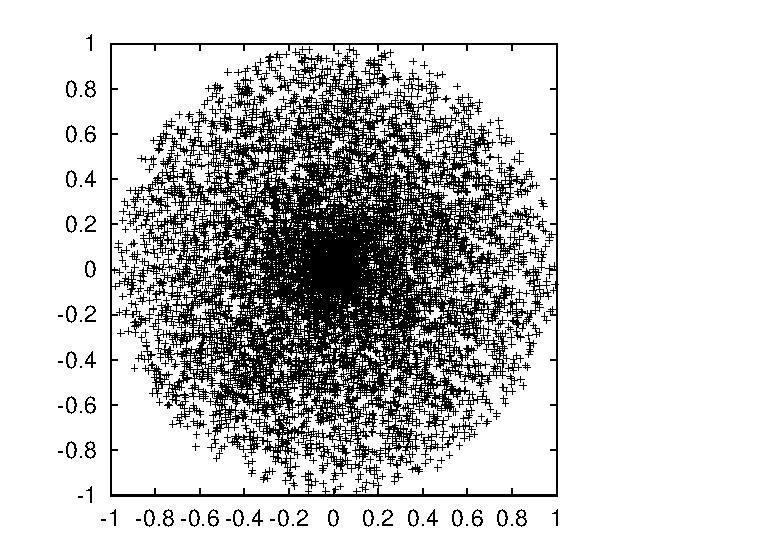
\includegraphics[width=4.5in]{chap9/test1axy10000.ps}
\caption[xy plot of {\st sphere1a} output]
{Output of {\st sphere1a}, with 10,000 particles, projected onto the
$\{x,y\}$ plane}
\label{fig:sphere1axy10000}
\end{figure}

\abc

\carol
(fig. \ref{fig:sphere1axy10000}) Looks good to me.  The particles are
closer together in the center than near the edge, but that must be
because we see more volume there, when we project the sphere on a
two-dimensional screen.

\alice
Yes, near the edge your line of sight only intersect a small sliver of
the sphere.  Although the density is homogeneous, that still gives you
only a few particles.

\bob
I guess we all believe our {\sl sphere.C} program to be correct now,
but just to make sure, let us plot another view, now that we have an
easy way to do that.

\carol
You are hard to satisfy!  But sure, why not.  Let take the $x$ and $z$
components of the positions, this time.

\alice
Okay, this is how to produce that picture:

\cba

\begin{small}
\begin{verbatim}
|gravity> gnuplot
Terminal type set to 'x11'
gnuplot> plot "test1a_10000.out" using 2:4 notitle
gnuplot>
\end{verbatim}
\end{small}

\begin{figure}[htb]
\centering
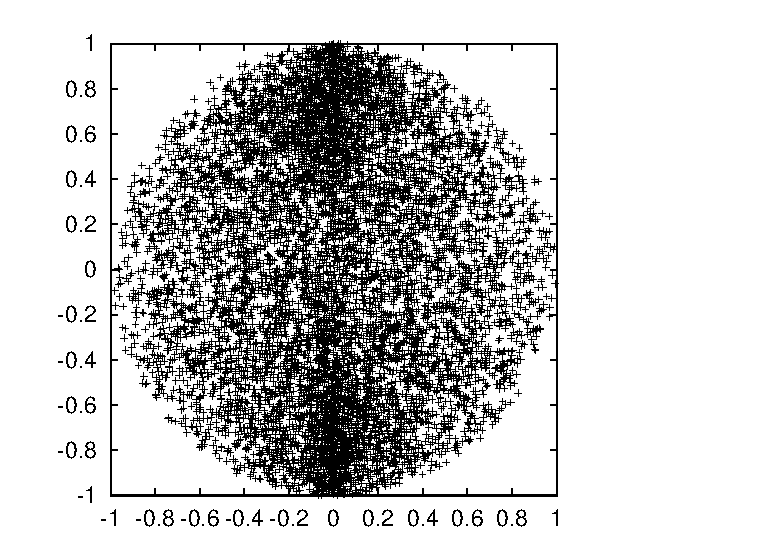
\includegraphics[width=4.5in]{chap9/test1axz10000.ps}
\caption[xz plot of {\st sphere1a} output]
{Output of {\st sphere1a}, with 10,000 particles, projected onto the
$\{x,z\}$ plane}
\label{fig:sphere1axz10000}
\end{figure}

\abc

\carol
(fig. \ref{fig:sphere1axz10000}) 
Wow!  That's weird!  What are those extra particles doing there, along
the vertical line in the middle of the picture?  That doesn't look at
all like a projection of a homogeneous sphere.

\bob
(smiling) So much for chiding me about testing too much.

\carol
Well, I must say, I'm glad now that you were hard to satisfy.  If you
wouldn't have insisted we would have moved right along.  Who knows how
long it would have taken us to find that bug, whatever it is \dots

\alice
\dots if we would have ever found it.  This is something scare about
using computers: you know you have done something wrong, when you see
that things don't look right, but the other way around does not hold.
Things can look pretty right all right, and still be wrong.

\bob
That reminds me of a philosopher, was it Popper, who said that you can
never verify a theory.  You can only falsify it.

\carol
Yes, that was him.  The best you can do is to make a theory more and
more plausible.  And yes, the same holds true for programming.  There
is a whole branch of computer science that deals with proving the
correctness of code.  However, they only talk about the internal
correctness of a code.  And that's the only thing they can possibly
talk about, since no compiler can ever test whether or not the
external information has been put in correctly.  If the physics input
is wrong, there is no logical way for any software program to find
that out.

\bob
True, although here we are really working with math more than physics,
assigning points to positions in space.  But I see your point.  Still,
physics is presumably consistent, so even there one can apply
consistency checks.

\carol
Yes, in a large system you must be right, but I'm not sure how far you
can get with such a small code as {\st sphere.C}.  It's a bit
embarrassing, frankly, to get such a wrong result with so few lines of
code.

\alice
Oh, believe me, I've made bigger mistakes in smaller codes.  But let's
put the philosophy aside for now, and let's fix things!  But first I
want to know precisely what's going on.  Let's take somewhat fewer
particles, and let us look at both picture again, just to have
another way of approach this mystery.

\carol
Here you are, with a thousand particles, instead of ten thousand.
First the $x$ and $y$ components of the positions.

\cba

\begin{small}
\begin{verbatim}
|gravity> sphere1a -n 1000 | tail +3 > test1a_1000.out
seed = 1063987133
|gravity> gnuplot
Terminal type set to 'x11'
gnuplot> plot "test1a_1000.out" using 2:3 notitle
gnuplot>
\end{verbatim}
\end{small}

\begin{figure}[htb]
\centering
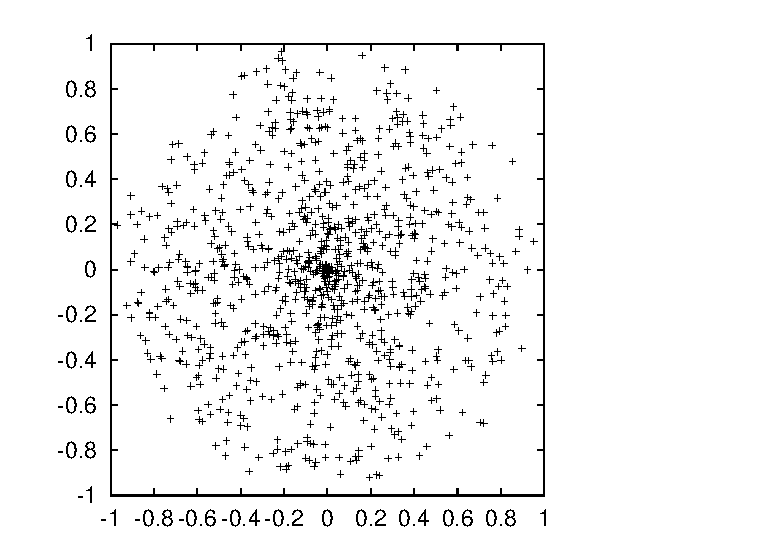
\includegraphics[width=4.5in]{chap9/test1axy1000.ps}
\caption[xy plot of {\st sphere1a} output]
{Output of {\st sphere1a}, with 1,000 particles, projected onto the
$\{x,y\}$ plane}
\label{fig:sphere1axy1000}
\end{figure}

\abc

\bob
(fig. \ref{fig:sphere1axy1000}) 
Now this looks okay again, as before.  However, I must say, I'm a
little puzzled by the fact that there are so many particles in the
center.  To have the density petering off toward the edge seems
reasonable, as we discussed a little earlier.  But why should there be
a spike in particle density near the center?

\carol
Good question.  Let's first look at the $\{x,z\}$ view.

\cba

\begin{small}
\begin{verbatim}
|gravity> gnuplot
Terminal type set to 'x11'
gnuplot> plot "test1a_1000.out" using 2:4 notitle
gnuplot>
\end{verbatim}
\end{small}

\begin{figure}[htb]
\centering
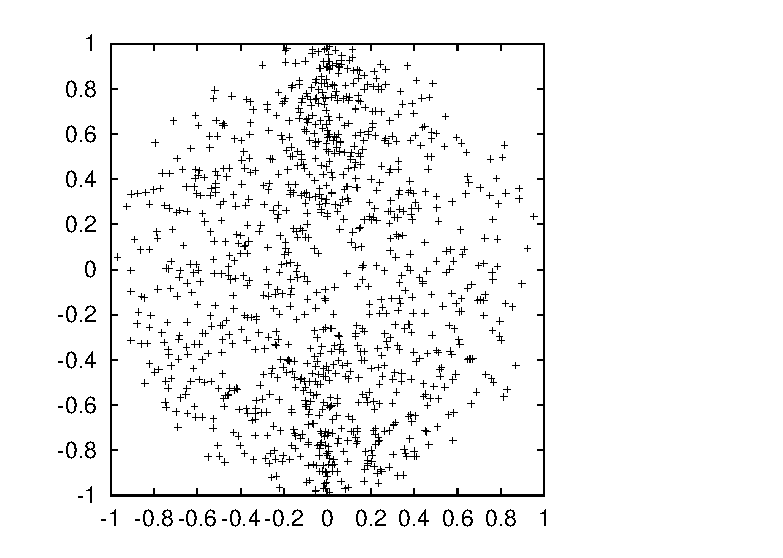
\includegraphics[width=4.5in]{chap9/test1axz1000.ps}
\caption[xz plot of {\st sphere1a} output]
{Output of {\st sphere1a}, with 1,000 particles, projected onto the
$\{x,z\}$ plane}
\label{fig:sphere1axz1000}
\end{figure}

\abc

\carol
(fig. \ref{fig:sphere1axz1000}) 
Same problem: too many particles near the central vertical.

\bob
Aha!  Now I can answer my own question.  Of course!  If there are
really too many particles near the central vertical line in the
$\{x,z\}$ plane, then that excess of particles will all be projected
near the center of the $\{x,y\}$ projection.

\alice
Good point indeed!  At least the bug we have found is consistent.
I am glad we are dealing with only one problem, rather than too!

\carol
But I would prefer to have no bug at all.  Let's have another look at
the code.

\cba

\section{Chasing the Bug}

\abc

\bob
Well, the one part which I must admit I did not fully understand is
where the angles are used to create particle positions in, what did
you call it again?

\alice
spherical coordinates.  A useful way to label particles by their
distance from the center, and by the two angles needed in addition to
locate them uniquely.

\carol
Useful, yes, if they do what they are supposed to do.  Bob may be right,
that is a likely place to have made a mistake.  Let us look at how
exactly we made that transformation.  Here is how we assigned the
positions and velocities to all the particles.

\cba

\code{sphere1a\_bugfragment.C: put\_snapshot}{chap9/sphere1a_bugfragment.C}

\abc

\alice
At first sight, it looks rather reasonable.  I clearly recognize the
spherical coordinate angles in the position assignments: the sines and
cosines of $\theta$ and $\phi$ are all in the right place.

\carol
And the ranges above those three lines are correct too: $\theta$ moves
from the north pole to the south pole, so to speak, which makes an arc
of $180^o$, starting at $\theta = 0$, as it should; similarly $\phi$
moves all the way around along the equator, describing an angle of $360^o$.
What could possibly be wrong?

\bob
Why are the $r$ values distributed according to a one-third power?

\alice
That's because the size of a volume element increases with the cube of $r$.
For example, if you double the radius of a three-dimensional object,
you make the volume eight times large.  In order to keep the same
density of points, you have to put eight times as many particles.

\bob
I see.  You want to distribute the particles uniformly random in $r^3$,
not in $r$.  So this means that $r$, which is the third root of $r^3$,
has to follow the third root of a uniformly distributed variable.

\alice
You got it.

\bob
And the angles don't need such a trick, because $r$ does not change
while we move around the latitude $\theta$ or the longitude $\phi$.

\alice
Right you are, that is indeed \dots OOPS \dots no \dots correction \dots
that is not indeed right, that is wrong.  Now I see our mistake!

\carol
But look, if you go around the equator, how can it make any difference
to where on the equator you are?

\alice
It doesn't, but try going to one of the poles.

\carol
Ah, now I get it.  Moving from the equator to the pole, the lines of
constant longitude converge together, and there is less and less room
between them, the closer you get to the pole.

\alice
And mathematically you express that by the expression for a volume
element $dV$ as:

\cba

\begin{equation}
d\:V \; = \; r^2 \sin \theta \; dr \; d\theta \; d\phi
\end{equation}

\abc
\alice
And for our application, it is easier to write this as
\cba

\begin{equation}
d\:V \; = \; d(\: r^3)\: \; d(\: cos \theta \:)\: \; d\phi
\end{equation}

\abc

\bob
So this means that we have to invert the cosine factor for $\theta$,
just as we inverted the third power for $r$ in the line above in our
code.

\alice
Exactly.  And the inverse of `$\cos \theta$' is `$\rm{acos}\, \theta$,
sometimes also written as `$\arccos \theta$.'  If we
sprinkle particles along latitude in such a way that we do it as the
arc cosine of $\theta$, we will no longer overpopulate the poles.

\carol
Ah, so that is what cause the crowding at the poles, something that
showed up only in the $\{x,z\}$ plot.

\bob
Because in the $\{x,y\}$ plot the poles are projected in the middle of
the equatorial plane.  The bug was less obvious there, although it did
create the spike in the center, which we all overlooked in the first
figure, which was a bit crowded with $10,000$ particles.

\alice
Well, I'm really glad we have found the bug, and it is easy to fix.
Let us call the corrected code {\st sphere1.C}.  The only difference
is the line for assigning random number values to $\theta$:

\cba

\begin{small}
\begin{verbatim}
|gravity> diff sphere1.C sphere1a.C
197c197
< 	real theta = acos(randinter(-1.0, 1.0));
---
> 	real theta = randinter(0.0, PI);
|gravity> 
\cba

\abc

\carol
Let's see whether things come out better.

\cba

\begin{small}
\begin{verbatim}
|gravity> sphere1 -n 1000 | tail +3 > test1_1000.out
seed = 1063988487
|gravity> gnuplot
Terminal type set to 'x11'
gnuplot> plot "test1_1000.out" using 2:3 notitle
gnuplot>
\end{verbatim}
\end{small}

\begin{figure}[htb]
\centering
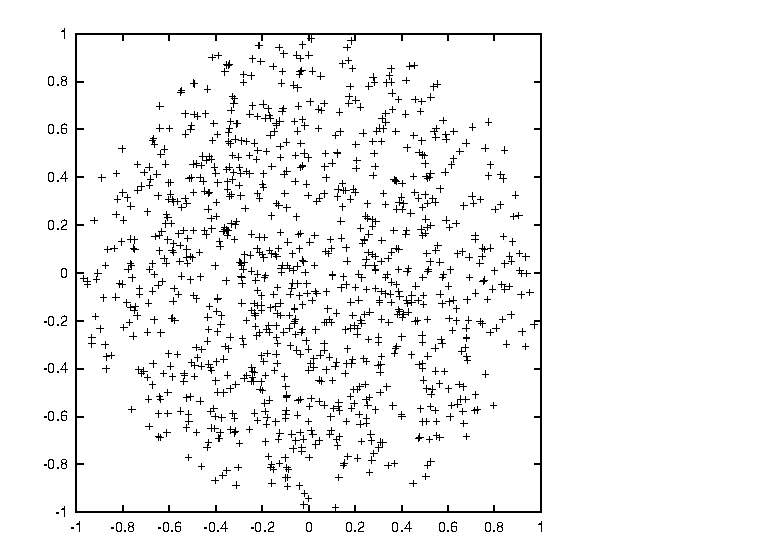
\includegraphics[width=4.5in]{chap9/test1xy1000.ps}
\caption[xy plot of {\st sphere1} output]
{Output of {\st sphere1}, with 1,000 particles, projected onto the
$\{x,y\}$ plane}
\label{fig:sphere1xy1000}
\end{figure}

\abc

\bob
(fig. \ref{fig:sphere1xy1000}) 
What a difference a line of code can make!  No spike in the center any
more.  Everything looks so much smoother.

\carol
Indeed.  There is only a mild edge effect, with somewhat fewer
particles far away from the center, but the contrast between center
and edge is much less than it was before.

\alice
This suggest that our central vertical line has cleared away.  Let's
make sure.

\cba

\begin{small}
\begin{verbatim}
|gravity> gnuplot
Terminal type set to 'x11'
gnuplot> plot "test1_1000.out" using 2:4 notitle
gnuplot>
\end{verbatim}
\end{small}

\begin{figure}[htb]
\centering
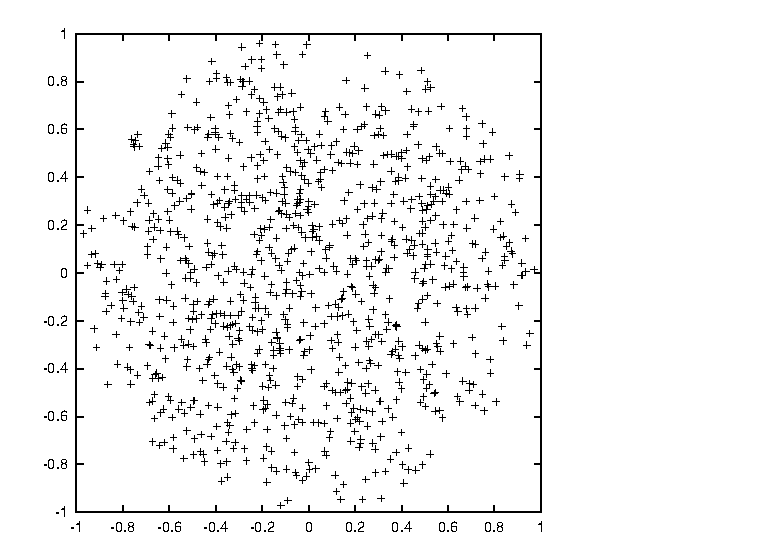
\includegraphics[width=4.5in]{chap9/test1xz1000.ps}
\caption[xz plot of {\st sphere1} output]
{Output of {\st sphere1}, with 1,000 particles, projected onto the
$\{x,z\}$ plane}
\label{fig:sphere1xz1000}
\end{figure}

\abc

\bob
(fig. \ref{fig:sphere1xz1000}) 
Indeed, a clean bill of health for {\st sphere1.C}

\carol
The moral of the story seems to be to try to test each module before
you start putting things together, no matter how tempting it is to
quickly write a few pieces and do some fun experiment with it.

\bob
Yes, and this must be equally true for real experiments as well as for
virtual experiments in cyberspace.  This reminds me of what I just
heard from a friend of mine, a graduate student in physics.  He talked
about an experiment he was involved in.  The wanted to test a new
magnet, to be used to deflect a particle beam, in his case a beam of
polarized electrons.  After finishing the construction of the magnet
setup, they bought a standard device that produced polarized electrons
of the right type, hooked it up to the magnet, and switched everything
on.  If all had gone well, fine, but in their case things did not go
well.  The result is not what they expected, and they didn't know at
that point whether there was something wrong with the magnet, with the
gadget producing the electrons, with the connection between the two
devices, or with the apparatus reading out the results (or even with
the operator of the equipment who might have had a bad day and
therefore made some kind of mistake).

\alice
It would have been worse, much worse actually, if all would have seemed
fine at first, but only because some subtle bug in one of the devices
produced an error that happened to be canceled more or less by another
error in another part of the setup.

\bob
That was his conclusion too.  He told me he realized that it is
crucially important to test one by one all the steps in constructing an
experimental setup.  The first step should have been to make sure that
the gadget generating the electrons is really doing what they expected
and hoped it would do.  In other words, they should first have carefully
measured the properties of the electron beam {\it before} it entered
the magnet setup.  Only when they really felt comfortable that their
gadget was working as advertised would it make sense to connect
it to the magnet, and to start analyzing the beam coming out of the
magnet.

\carol
I think the analogy is a good one, and that what is true for a
traditional lab is true for our virtual lab as well.  We did not
really confront this problem earlier, since we dealt only with two or
three particles, for which we wrote the initial conditions by hand.  In
contrast, we now have reached a point where for the first time we are
generating initial conditions automatically.  And anything that is
done automatically can go wrong in all kind of unexpected ways.

\alice
Well, it is still possible to make mistakes when entering numbers
by hand.  I sure have done that more often than I'd like to admit.

\carol
Of course, but when you are dealing with a two-body or three-body
system, you can track the orbits individually on the screen, and if
you are careful, you will notice if the particles behave completely
different from what you expected.  But as soon as we start generating
initial conditions automatically in large numbers, for a 25-body
system for example, the situation is drastically different.  It is no
longer possible to look at the spaghetti of tangled orbits on a screen
and to decide whether all 25 particles do even remotely what they are
supposed to do.  And indeed, the whole reason to use a computer,
rather than pen and paper, is to solve a problem that is too complex
to predict analytically beforehand.  So you don't know in detail
what to expect, and you may not notice if any part of the system
behaves differently from how it should behave.

\bob
I bet your must have heard about modular testing in one of your
computer science classes.

\carol
Yes, but frankly I thought they exaggerated a bit.  The typical home
work problems were often so simple that it was easy to see whether
you got it right or not.  But with our example today, I can see how
essential it is to test each and every module you write, before
hooking it up to other modules.  If you test modules one by one, then
it is most likely that a new bug in a complex of modules is generated
by the latest module you have just added; or at least is caused by an
unexpected interaction between that new module and what was already
tested before.  In both cases, you are far better off than if you
suddenly have to test a whole conglomeration of modules, where errors
could be hidden in any of them.

\alice
That last scenario is a nightmare, and a good way to quickly loose
interest in computer programming.

\cba

\begin{Exercise}[Rejection technique]\label{ex:rejectiontechnique}
Inspect the following code.  It uses a completely different technique
to generate initial conditions for a homogeneous sphere.  It is
simpler in that it does not use any trigonometric functions, but only
the usual Cartesian coordinates.  This sounds almost too good to be
true. Can you figure out how the rejection technique works?  Try it
out and compare its results with that of {\st sphere1.C}.
\end{Exercise}

\code{sphere2.C}{chap9/sphere2.C}

